\begin{frame}[fragile]{Results: Randomisation Drive Task} % some commands, e.g. \verb require [fragile]
\begin{figure}
  \centering
  \subfloat{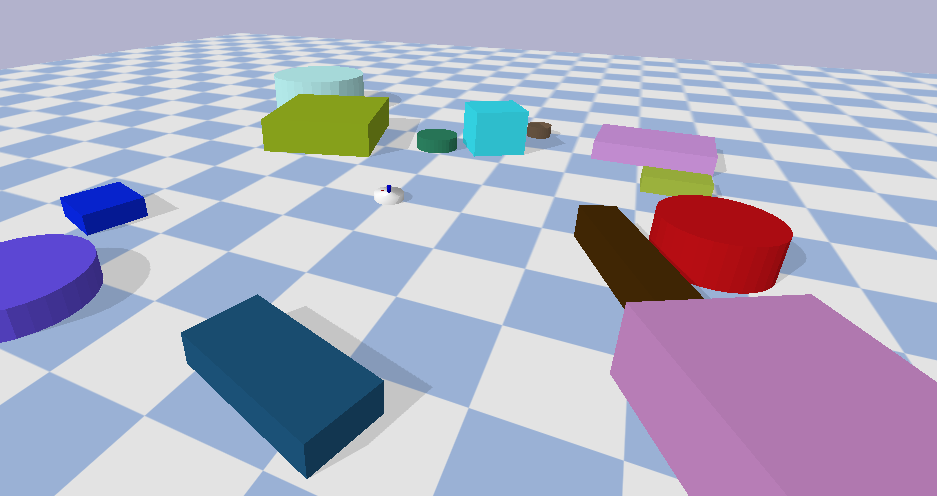
\includegraphics[width=0.45\textwidth]{figures/results/random1}}\quad
  \subfloat{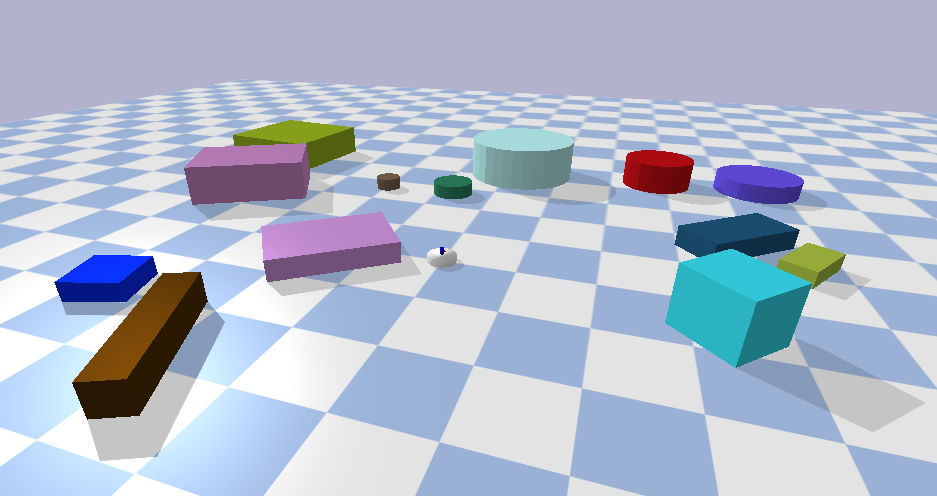
\includegraphics[width=0.45\textwidth]{figures/results/random2}}
\end{figure}
\vspace{-0.7cm}
\begin{figure}
  \centering
  \subfloat{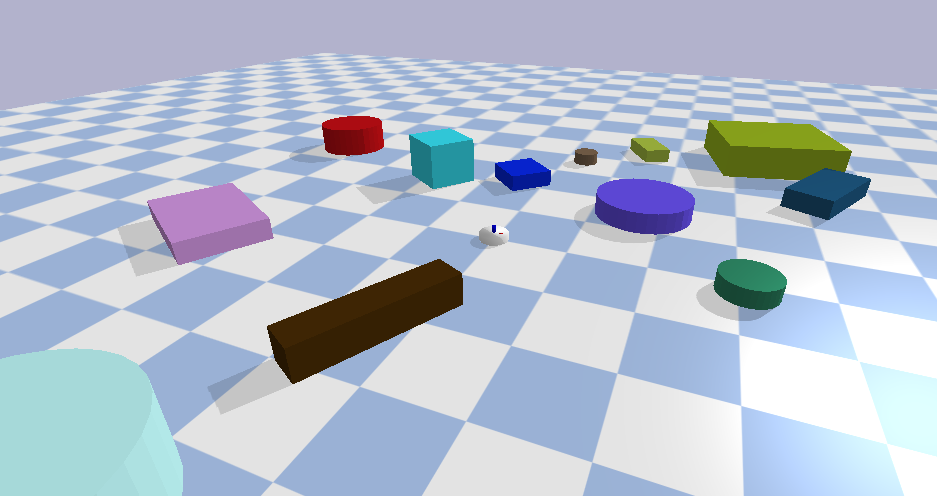
\includegraphics[width=0.45\textwidth]{figures/results/random3}}\quad
  \subfloat{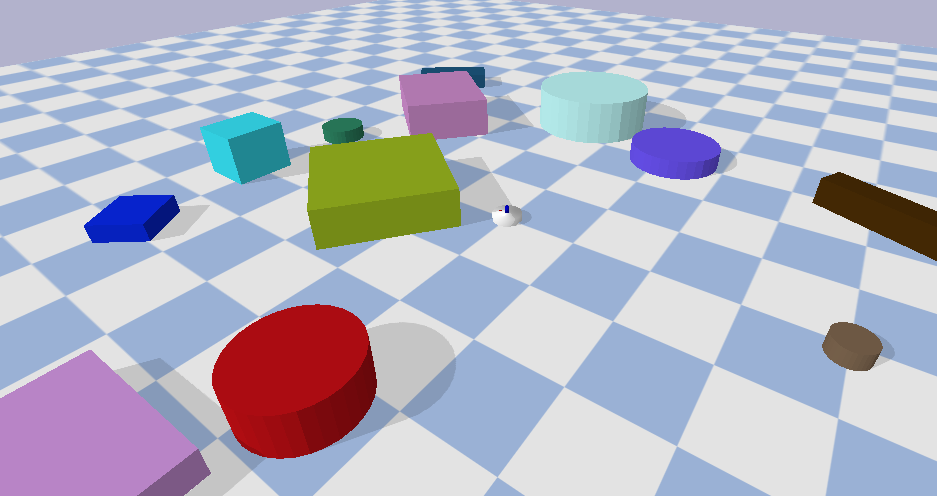
\includegraphics[width=0.45\textwidth]{figures/results/random4}}
\end{figure}
\end{frame}


\begin{frame}[fragile]{Results: Randomisation Push Task} % some commands, e.g. \verb require [fragile]
\begin{center}
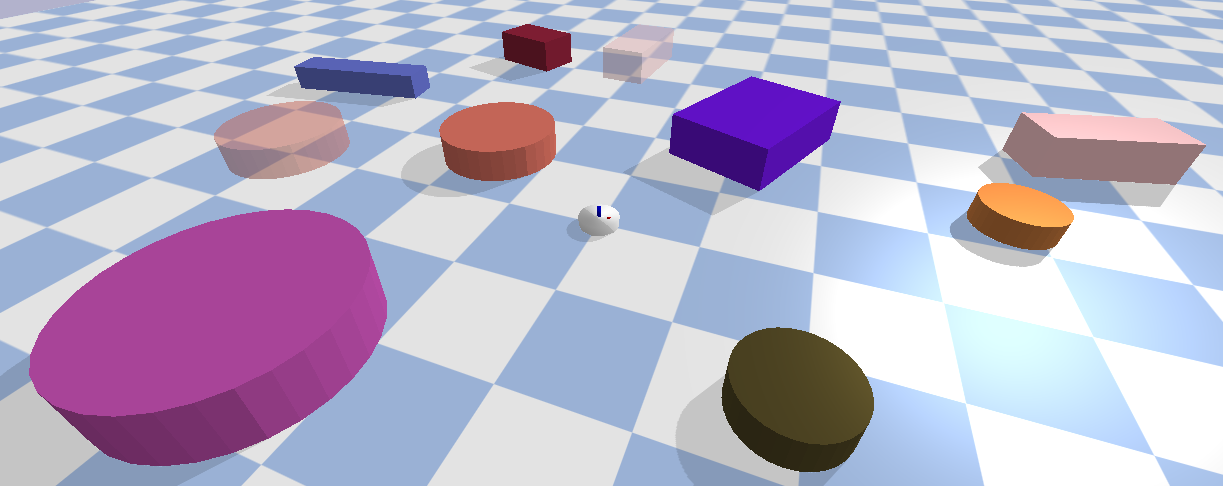
\includegraphics[width=1.0\textwidth]{figures/results/random_1}
\end{center}
\end{frame}

\begin{frame}[fragile]{Results: Randomisation Drive Task Execution Times} % some commands, e.g. \verb require [fragile]
\begin{center}
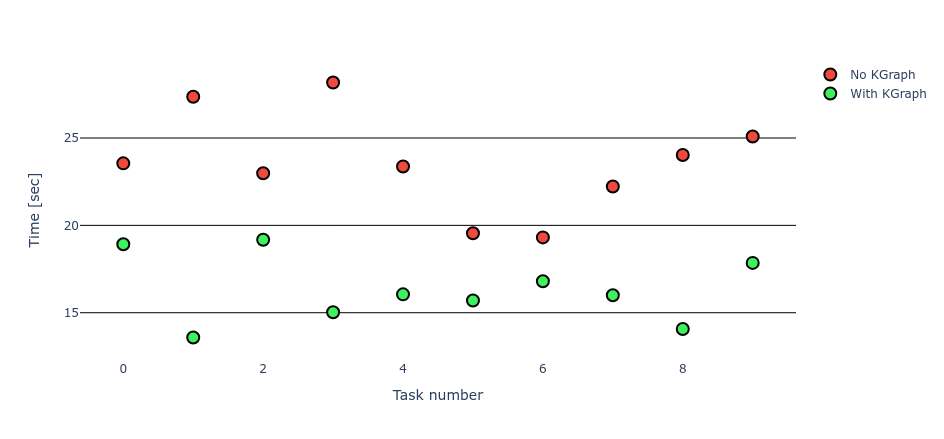
\includegraphics[width=1.0\textwidth]{figures/results/random_drive_time_vs}
\end{center}
\end{frame}

\begin{frame}[fragile]{Results: Randomisation Push Task Execution Times} % some commands, e.g. \verb require [fragile]
\begin{center}
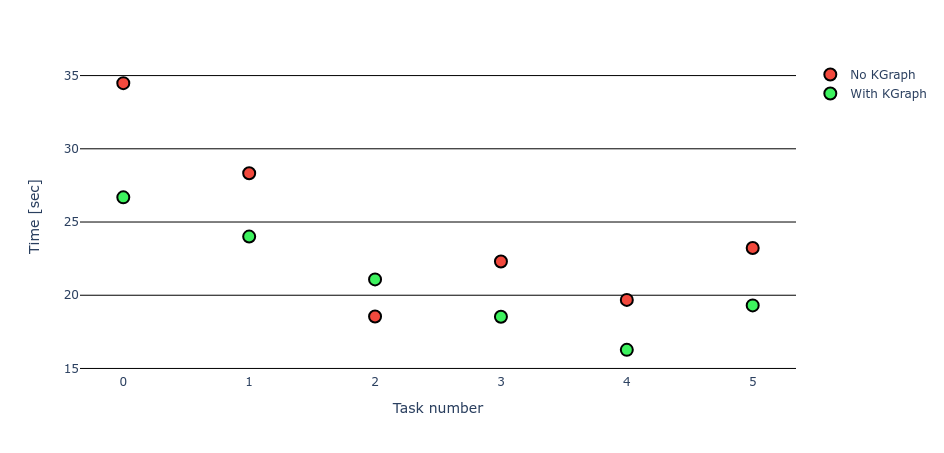
\includegraphics[width=1.0\textwidth]{figures/results/random_push_time_vs}
\end{center}
\end{frame}

\begin{frame}[fragile]{Results: Randomisation Push Task Prediction Error} % some commands, e.g. \verb require [fragile]
\begin{center}
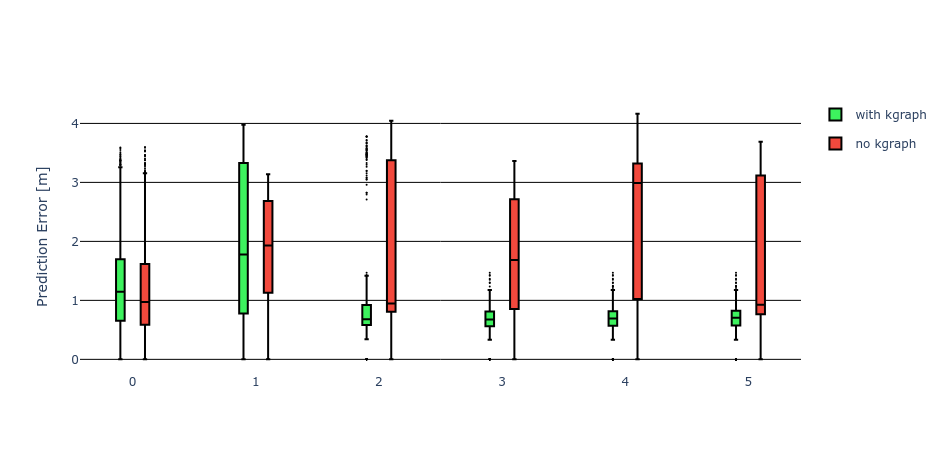
\includegraphics[width=1.0\textwidth]{figures/results/random_push_pe_vs}
\end{center}
\end{frame}

\begin{frame}[fragile]{Results} % some commands, e.g. \verb require [fragile]
\begin{table}[H]
  \centering
  \begin{tabular}
  {>{\raggedright\arraybackslash}p{2.0cm}%
    ccc%
    >{\raggedright\arraybackslash}p{2.5cm}}
    Author &  Learning & NAMO & Object to Target & Manipulation\\[2mm]
    \citeauthor{ellis_navigation_2022}  &\cmark& \cmark& \xmark& pushing\\
    \citeauthor{sabbaghnovin_model_2021} & \cmark& \xmark& \cmark& grasp-push grasp-pull\\
    \citeauthor{scholz_navigation_2016} & \cmark& \cmark& \xmark& graph-push grasp-pull\\
    \citeauthor{vega-brown_asymptotically_2020} & \xmark& \cmark& \cmark& gripping\\[2mm]
    \citeauthor{wang_affordancebased_2020} & \cmark& \cmark& \xmark& pushing\\
    Groote & \xmark/\cmark & \cmark & \cmark & pushing\\
  \end{tabular}
\end{table}
\end{frame}

\begin{frame}[fragile]{More convincing environments}
\begin{figure}
  \centering
  \subfloat{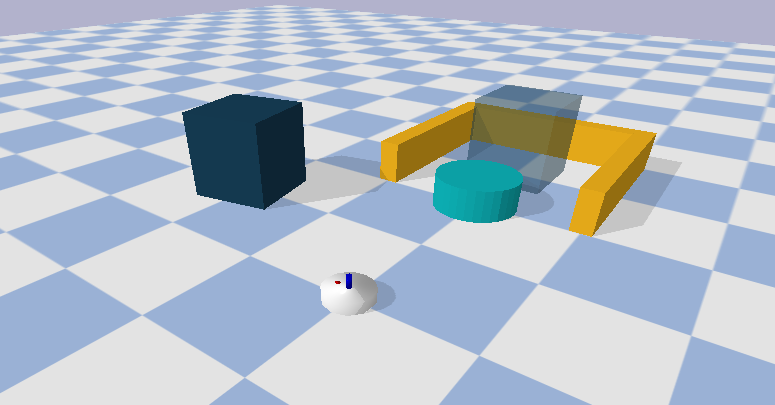
\includegraphics[width=0.45\textwidth]{figures/results/blockade}}\quad
  \subfloat{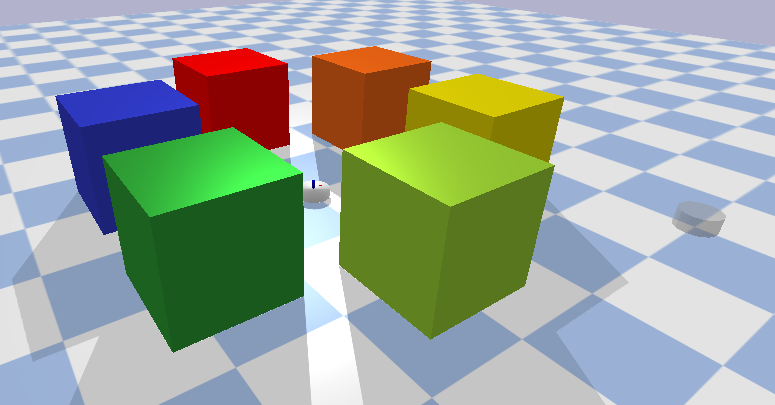
\includegraphics[width=0.45\textwidth]{figures/results/surrounded}}
\end{figure}
\vspace{-0.7cm}
\begin{figure}
  \centering
  \subfloat{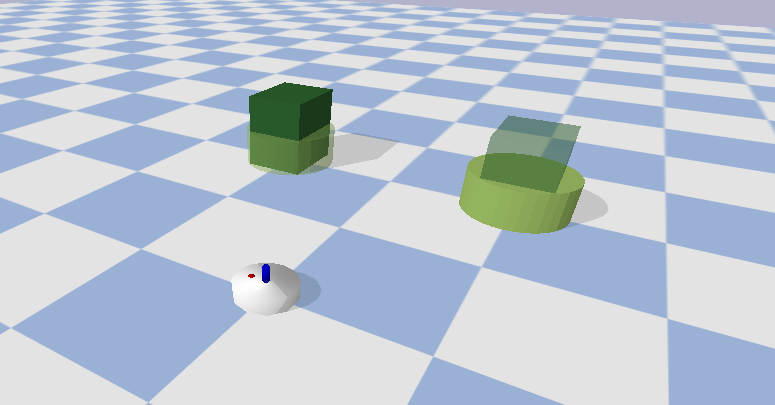
\includegraphics[width=0.45\textwidth]{figures/results/swap}}\quad
  \subfloat{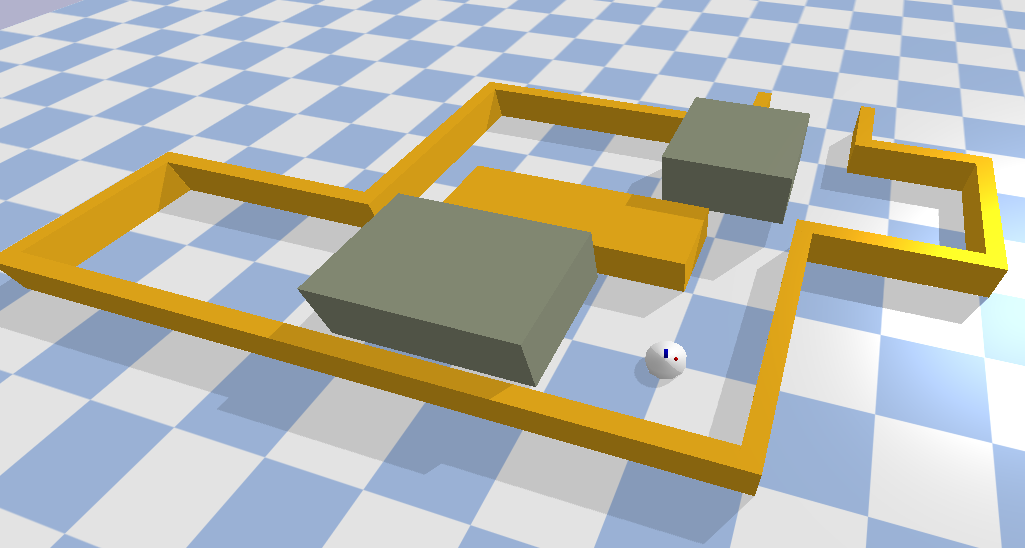
\includegraphics[width=0.45\textwidth]{figures/introduction/2_pushes_to_freedom}}
\end{figure}

\end{frame}


\begin{frame}[fragile]{4 Week Planning}
  \begin{block}{Good Scenario}
    \begin{itemize}
      \item 50 \% Report \\
      \item 50 \% Presentation
    \end{itemize}
  \end{block}\pause

  \begin{exampleblock}{Better Scenario}
    \begin{itemize}
      \item 40 \% Report \\
      \item 40 \% Presentation \\
      \item 20 \% Benchmark Environments
    \end{itemize}
   \end{exampleblock}
\end{frame}


